\chapter{System analysis and design}
\section{System analysis}
\noindent
As indicated earlier, the system was developed in three major iterations. However, before the
iterations had begun, initial requirement gathering and analysis was done. This covered the whole
system.
\subsubsection{Initial requirement gathering and analysis}
Functional requirements:
Nonfunctional requirements:
Constraints (“Pseudo requirements”):
\subsection{Iteration 1}
This iteration involved the development of the web crawler module of the system.
\subsubsection{Requirements}
\subsubsection{Functional requirements}
\begin{itemize}
\item Crawl webpages in any domain given a base url
\item Take into account rich files i.e. pdf, doc,xls,
\item Discard similar pages
\item Resilient to network outages (saves state)
\end{itemize}
\subsubsection{Non-functional requirements}
\begin{enumerate}
\item Minimal traffic
\item Not overload servers
\item Able to start/pause/resume/stop/resume on demand
\item Avoid getting banned
\end{enumerate}

\subsection{Iteration 2}
This iteration involved the development of the data analysis module.

\subsection{Iteration 3}
This iteration involved the development of the data presentation module

\subsection{Usecases}
\begin{figure}
	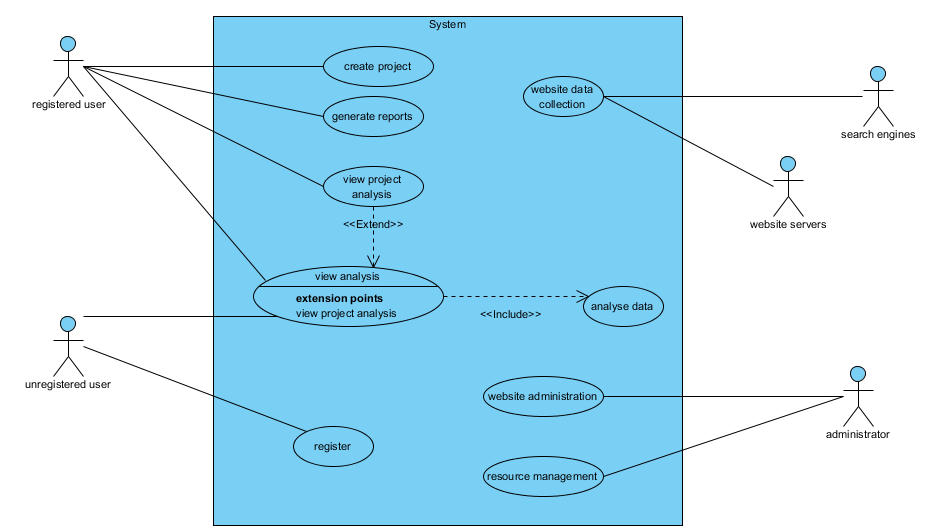
\includegraphics[width=\linewidth]{usecase.png}
	\caption{System use case model}
\end{figure}

\subsubsection{Usecase 1}
\begin{table}[H]
\centering
\begin{tabular}{|l|l|}
\hline
    \thead{Name} & Create project\\
\hline
    \thead{Id} & 1\\
\hline
    \thead{Version} & 1\\
\hline
    \thead{Summary} & Create new webometric analysis project\\
\hline
    \multirow{2}{*}{\thead{Actors}} & User\\
            & System\\
\hline
    \multirow{3}{*}{\thead{Entry conditions}} & User is registered\\
            & User is logged in\\
            & University domains are presented to user\\
\hline
    \thead{Exit conditions} & System starts data collection\\
\hline
    \thead{Triggers} & \\
\hline
\end{tabular}
\caption{Use case 1}
\end{table}

\subsubsection{Flow of events}
\subsubsection{Basic flow of events}
\begin{enumerate}
\item User enters the project name
\item User chooses domain to analyse
\item System notifies the user that the project started successfully
\item System starts website data collection
\end{enumerate}

\subsubsection{Alternate flow of events}
A1 Server down
\paragraph{}
Server is unable to respond to client requests. The client is notified of this and asked to retry again later.
\linebreak
A2 Alternate domain
\paragraph{}
User enters domain and start URL manually instead of choosing from the available ones. The domain entered should be a subdomain of the available domains.


\subsubsection{Scenario matrix}
\begin{table}[H]
\centering
\begin{tabular}{|l|l|l|}
\hline
    \thead{Name} & \thead{Starting flow} & \thead{Alternate flow} \\
\hline
    Project created successfully & Basic flow & \\
\hline
    Server down & Basic flow  & A1 \\
\hline
\end{tabular}
\caption{scenario matrix for usecase 1}
\end{table}


\subsubsection{Usecase 2}
\begin{table}[H]
\centering
\begin{tabular}{|l|l|}
\hline
    \thead{Name} & View analysis\\
\hline
    \thead{Id} & 2\\
\hline
    \thead{Version} & 1\\
\hline
    \thead{Summary} & View analysis of domains whose data is already in the system\\
\hline
    \multirow{2}{*}{\thead{Actors}} & User\\
            & System\\
\hline
    \multirow{2}{*}{\thead{Entry conditions}}
            & Domains whose data is collected are presented to the user\\
            & Domain data is collected\\
\hline
    \thead{Exit conditions} & User views analyses of selected domains\\
\hline
    \thead{Triggers} & \\
\hline
\end{tabular}
\caption{Use case 2}
\end{table}

\subsubsection{Flow of events}
\subsubsection{Basic flow of events}
\begin{enumerate}
\item User chooses domains whose data is already collected
\item System generates results
\item System presents results to user
\end{enumerate}

\subsubsection{Alternate flow of events}
A1 Server down
\paragraph{}
Server is unable to respond to client requests. The client is notified of this and asked to retry again later.
\linebreak


\subsubsection{Usecase 3}
\begin{table}[H]
\centering
\begin{tabular}{|l|l|}
\hline
    \thead{Name} & View project analysis\\
\hline
    \thead{Id} & 3\\
\hline
    \thead{Version} & 1\\
\hline
    \thead{Summary} & View analysis of a project created by the user\\
\hline
    \multirow{2}{*}{\thead{Actors}} & User\\
            & System\\
\hline
    \multirow{3}{*}{\thead{Entry conditions}} & User is registered\\
            & Project is started by user\\
            & Data is analysed\\
\hline
    \thead{Exit conditions} & User views analysis\\
\hline
    \thead{Triggers} & \\
\hline
\end{tabular}
\caption{Use case 3}
\end{table}

\subsubsection{Flow of events}
\subsubsection{Basic flow of events}
\begin{enumerate}
\item System fetches analysis
\item User views analysis
\end{enumerate}

\subsubsection{Alternate flow of events}
A1 Server down
\paragraph{}
Server is unable to respond to client requests. The client is notified of this and asked to retry again later.
\linebreak


\subsubsection{Usecase 4}
\begin{table}[H]
\centering
\begin{tabular}{|l|l|}
\hline
    \thead{Name} & Generate project reports\\
\hline
    \thead{Id} & 4\\
\hline
    \thead{Version} & 1\\
\hline
    \thead{Summary} & User generates reports based on the data collected in the project\\
\hline
    \multirow{2}{*}{\thead{Actors}} & User\\
            & System\\
\hline
    \multirow{3}{*}{\thead{Entry conditions}} & User is registered\\
            & Project started by user\\
            & Website data collected\\
            & Data analysed\\
\hline
    \thead{Exit conditions} & User generates reports\\
\hline
    \thead{Triggers} & \\
\hline
\end{tabular}
\caption{Use case 4}
\end{table}

\subsubsection{Flow of events}
\subsubsection{Basic flow of events}
\begin{enumerate}
\item System presents results to user
\item User chooses results to include in report
\item System generates report and presents to user
\end{enumerate}

\subsubsection{Alternate flow of events}
A1 Server down
\paragraph{}
Server is unable to respond to client requests. The client is notified of this and asked to retry again later.


\subsubsection{Usecase 5}
\begin{table}[H]
\centering
\begin{tabular}{|l|l|}
\hline
    \thead{Name} & Register\\
\hline
    \thead{Id} & 5\\
\hline
    \thead{Version} & 1\\
\hline
    \thead{Summary} & An unregistered user registers with the system\\
\hline
    \multirow{2}{*}{\thead{Actors}} & User\\
            & System\\
\hline
    \thead{Entry conditions} & User is unregistered\\
\hline
    \thead{Exit conditions} & User is registered\\
\hline
    \thead{Triggers} & \\
\hline
\end{tabular}
\caption{Use case 5}
\end{table}

\subsubsection{Flow of events}
\subsubsection{Basic flow of events}
\begin{enumerate}
\item User enters username, email and password
\item System creates user account
\item System sends user an email with confirmation link via the given email address
\item System notifies user to confirm email address using confirmation link
\item User checks their email and clicks the confirmation link
\item System confirms account
\item System notifies user account confirmation successful
\end{enumerate}

\subsubsection{Alternate flow of events}
A1 Server down
\paragraph{}
Server is unable to respond to client requests. The client is notified of this and asked to retry again later.
\linebreak
A2 Username taken
\paragraph{}
The user is asked to pick another username.
\linebreak
A3 Email taken
\paragraph{}
The user is asked to pick another email address.
\linebreak
A4 Email not confirmed
\paragraph{}
The user is asked to confirm email address


\subsubsection{Usecase 6}
\begin{table}[H]
\centering
\begin{tabular}{|l|l|}
\hline
    \thead{Name} & Website data collection\\
\hline
    \thead{Id} & 6\\
\hline
    \thead{Version} & 1\\
\hline
    \thead{Summary} & The system fetches data about a specific domain\\
\hline
    \multirow{2}{*}{\thead{Actors}} & System\\ & Website servers\\ & Search engines\\
\hline
    \thead{Entry conditions} & Domain data is not existent\\
\hline
    \thead{Exit conditions} & Domain data collected\\
\hline
    \thead{Triggers} & Create project\\
\hline
\end{tabular}
\caption{Use case 6}
\end{table}

\subsubsection{Flow of events}
\subsubsection{Basic flow of events}
\begin{enumerate}
\item Website servers from chosen domains serve web pages
\item Search engines provide data about chosen domains
\item System analyses data collected
\item System generates results
\item User views results
\end{enumerate}

\subsubsection{Alternate flow of events}
A1 Server down
\paragraph{}
Server is unable to respond to client requests. The client is notified of this and asked to retry again later.
\linebreak
A2 Maximum concurrent crawls exceeded
\paragraph{}
The new crawl request is left pending waiting for a running one to finish.
\linebreak
A3 Data present
\paragraph{}
Data for the chosen domain is present and upto date
\linebreak

\subsubsection{Usecase 7}
\begin{table}[H]
\centering
\begin{tabular}{|l|l|}
\hline
    \thead{Name} & Analyse data\\
\hline
    \thead{Id} & 7\\
\hline
    \thead{Version} & 1\\
\hline
    \thead{Summary} & System analyses data collected from websites and search engines\\
\hline
    \thead{Actors} & System \\
\hline
    \thead{Entry conditions} & Data collected\\
\hline
    \thead{Exit conditions} & Data analysed\\
\hline
    \thead{Triggers} & Data collected\\
\hline
\end{tabular}
\caption{Use case 7}
\end{table}

\subsubsection{Flow of events}
\subsubsection{Basic flow of events}
\begin{enumerate}
\item Analyze data collected for the project
\item Generate results for the project
\item Send project's creator an email notifying them of availability of results
\end{enumerate}
\subsubsection{Alternate flow of events}


\section{System design}

\subsubsection{Context diagram (Level 0 DFD)}
\begin{figure}[H]
	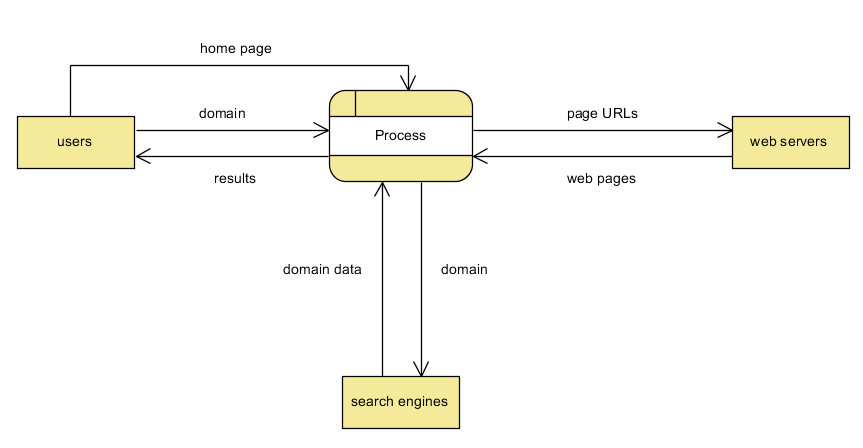
\includegraphics[width=\linewidth,scale=0.5]{../static/img/contextdiagram.png}
	\caption{Level 0 DFD}
\end{figure}

\subsubsection{Level 1 DFD}
\begin{figure}[H]
	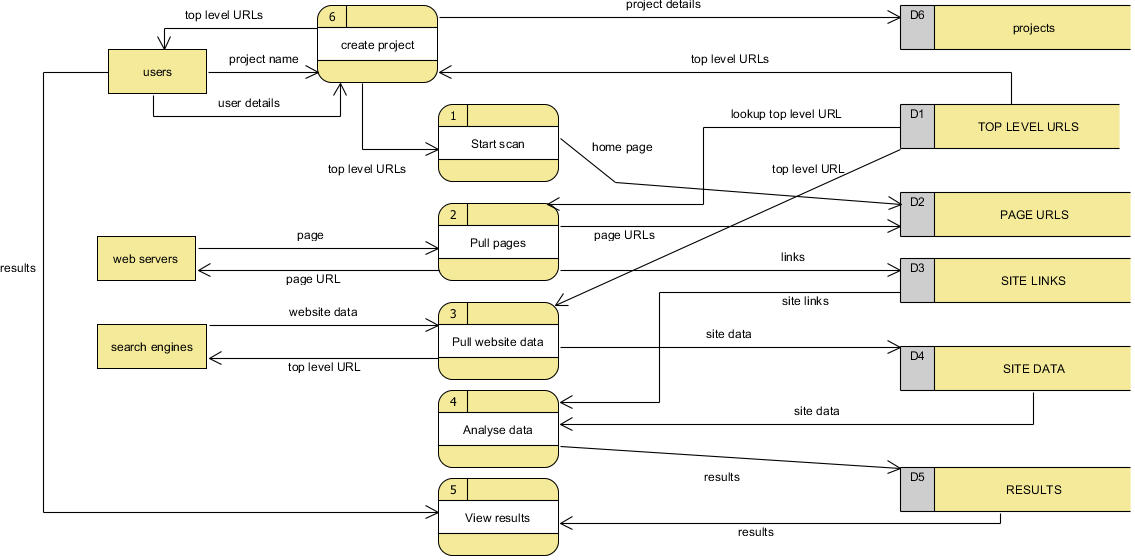
\includegraphics[width=\linewidth,scale=0.5]{../static/img/level_1_dfd.png}
	\caption{Level 1 DFD}
\end{figure}

\subsection{Web crawler design}
\begin{figure}[H]
	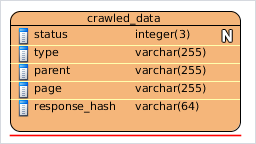
\includegraphics[width=\linewidth,scale=0.5]{../static/img/crawler_datastore.png}
	\caption{Webcrawler datastore design}
\end{figure}
\begin{figure}[H]
	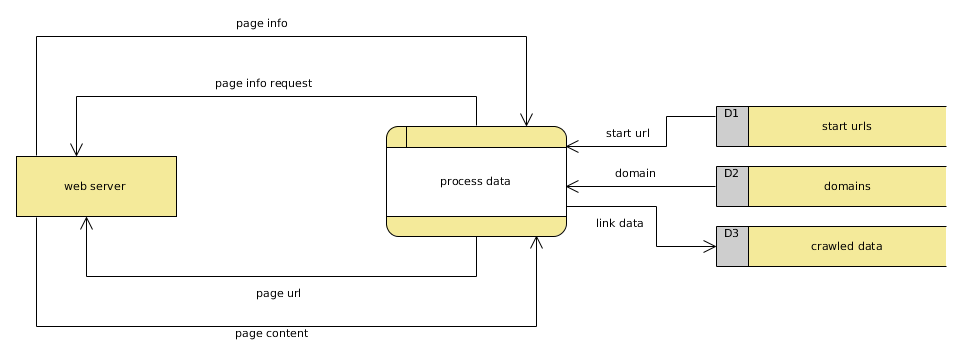
\includegraphics[width=\linewidth,scale=0.5]{../static/img/crawler_level1_dfd.png}
	\caption{Webcrawler DFD}
\end{figure}

\begin{table}[H]
\centering
\begin{tabular}{|l|c|}
\hline
    \thead{Item} & \thead{Description}\\
\hline
    Status & Status of the page being analysed e.g. 200 (available), 404 (not available)\\
\hline
    Type & Content type of resource being analysed e.g. text/html (html resource)\\
\hline
    Response hash & Hash of web resource being analysed\\
\hline
    Parent & URL of web resource being analysed\\
\hline
    Page & URL of web link extracted from content in web page being analysed\\
\hline
\end{tabular}
\caption{Web crawler data dictionary}
\end{table}

